\documentclass[a4paper, 12pt, final, garamond]{book}
\usepackage{cours-preambule}

\raggedbottom

\makeatletter
\renewcommand{\@chapapp}{Ondes -- chapitre}
\makeatother

\begin{document}
\setcounter{chapter}{1}

\chapter{Correction du TD}
\section{Interférences de 2 ondes sonores frontales}

\begin{enumerate}
    \item À partir de HP1, les ondes parcourent la distance $D+x$ pour arriver
        au micro. À partir de HP2, elles parcourent la distance $D-x$. Ainsi,
        \begin{align*}
            \D\f_{1/2}(\Mr)
                &= -k\D L_{1/2}(\Mr) + \underbrace{\D\f_0(\Mr)}_
                    {\mathclap{= 0 \text{ d'après l'énoncé}}}
            \\
                &= - k \left( {\rm \abs{HP_1M} - \abs{HP_2M}} \right)
            \\
                &= - k \left( \cancel{D}+x - (\cancel{D}-x) \right)
            \\
            \Leftrightarrow
            \Aboxed{
            \D\f_{1/2}(\Mr)
                &= - 2kx}
        \end{align*}

    \item Les ondes $p_1$ et $p_2$ étant de même amplitude $P_0$, on a que
        l'onde somme $p(t) = p_1(t) + p_2(t)$ est d'amplitude $P$ telle que
        \[P = 2P_0\cos(\frac{\D\f(\Mr)}{2})
        \Leftrightarrow
        \boxed{P = 2P_0\cos(-kx)}\]
    \item On a interférences constructives si l'amplitude est maximale, ici pour
        $\cos(-kx_n) = \pm 1 \Leftrightarrow -kx_n = n\pi$. Or,
        \begin{gather*}
            -kx_n = n\pi
            \Leftrightarrow
            - \frac{2\cancel{\pi}}{\lambda}x_n = n\cancel{\pi}
            \Leftrightarrow
            \boxed{
            x_n = n \frac{\lambda}{2}}
        \end{gather*}
    \item Les maximums se trouvent aux positions $x_n$. La distance entre deux
        maximums est donc
        \begin{gather*}
            \boxed{d = x_{n+1} - x_n = \frac{\lambda}{2}}
        \end{gather*}
    \item Étant donné que $\lambda = cT = c/f$, on trouve
        \begin{gather*}
            \frac{\lambda}{2} = d
            \Leftrightarrow
            \frac{c}{2f} = d
            \Leftrightarrow
            \boxed{c = 2df}
            \qavec
            \left\{
                \begin{array}{rcl}
                    d & = & \SI{21.2e-2}{m}\\
                    f & = & \SI{800}{Hz}
                \end{array}
            \right.\\
            \mathrm{A.N.~:}\quad
            \boxed{c = \SI{339}{m.s^{-1}}}
        \end{gather*}
        C'est la valeur usuelle de célérité du son dans l'air à
        \SI{20}{\degreeCelsius}.
\end{enumerate}

\section{Interférences sur la cuve à ondes}
\begin{enumerate}
    \item Par définition,
        \begin{gather*}
            \D\f_{1/2}(\Mr) = -k\D L_{1/2}(\Mr) = -k(d_1 - d_2) =
            \frac{2\pi}{\lambda}(d_2-d_1)
        \end{gather*}
        Et pour avoir des interférences destructives,
        \begin{gather*}
            \D\f_{1/2}(\Mr) = (2m+1)\pi
            \Leftrightarrow
            \frac{2\cancel{\pi}}{\lambda}(d_2-d_1) = (2m+1)\cancel{\pi}
            \Leftrightarrow
            \boxed{d_2-d_1 = \left(m+\frac{1}{2}\right)\lambda}
        \end{gather*}
    \item Avec ${\rm S_1S_2} = a$, on observe que tout l'axe $x > a/2$
        correspond à une ligne de vibration minimale, c'est-à-dire un endroit de
        l'espace où les interactions sont destructives, i.e. $d_2-d_1 =
        (m+1/2)\lambda$. Or, pour $x > a/2$, on a
        \begin{gather*}
            d_2 - d_1 = {\rm S_2M} - {\rm S_1M}
            = \cancel{\rm S_2M} - {\rm S_1S_2} + \cancel{\rm S_2M}
            \Leftrightarrow
            \boxed{d_2 - d_1 = -a}
        \end{gather*}
        On en déduit donc
        \begin{gather*}
            \boxed{\abs{\frac{a}{\lambda}} = m+\frac{1}{2}}
        \end{gather*}
        c'est-à-dire que $a/\lambda$ est un demi-entier (1/2, 3/2, 5/2…). Le
        résultat est le même en raisonnant sur $x < -a/2$.
    \item Entre $\rm S_1$ et $\rm S_2$, on prend 3 cas extrêmes pour déterminer
        l'amplitude de $d_2 - d_1$~:
        \begin{itemize}
            \item En $\rm S_1$, $d_2 = -a$ et $d_1 = 0$, donc
                \[d_2 - d_1 = -a\]
            \item En O, $d_2 = -a/2$ et $d_1 = a/2$, donc
                \[d_2 - d_1 = 0\]
            \item En $\rm S_2$, $d_2 = 0$ et $d_1 = a$, donc
                \[d_2 - d_1 = -a\]
        \end{itemize}
        Ainsi,
        \begin{gather*}
            \boxed{-a \leqslant d_2 - d_1 \leqslant a}
        \end{gather*}
        Or, entre $\rm S_1S_2$ on observe plusieurs vibrations minimales,
        donnant chacune $d_2 - d_1 = (m+\frac{1}{2})\lambda$. On en compte 8
        entre $\rm S_1S_2$, correspondant chacune à un ordre d'interférence $m$.
        À partir de O et vers les $x$ croissants, on a la première vibration
        minimale pour $m=0$, la deuxième pour $m=1$, la troisième pour $m=2$ et
        la dernière pour $m=3$~; on a de même par symétrie vers les $x$
        décroissants. Ainsi, \textbf{l'ordre d'interférence obtenu le plus grand
        est $m=3$}, et \textbf{on n'a pas l'ordre d'interférence $m=4$} sinon on
        aurait une parabole en plus de chaque côté. Ainsi,
        \begin{gather*}
            \left(3+\frac{1}{2}\right)\lambda
            < a \leqslant
            \left(4+\frac{1}{2}\right)\lambda
        \end{gather*}
        puisqu'on observe qu'il reste une distance sur $\rm S_1S_2$ après
        l'ordre 3 avant d'atteindre S$_2$ et que si $a$ dépasse $(4+1/2)\lambda$
        on verrait la parabole correspondant à l'ordre 4. Comme on a déterminé à
        la question précédente que $\frac{a}{\lambda} = m + \frac{1}{2}$, avec
        cette étude on a $3 < m \leqslant 4$ avec $m \in \Nb$, autrement dit
        \fbox{$m = 4$}, soit
        \[\boxed{\frac{a}{\lambda} = \frac{9}{2}}\]
    \item Le contraste correspond à une grande différence entre les valeurs
        maximales et minimales. Or, sur (O$y$) on a $d_2 = d_1$ donc $d_2-d_1 =
        0$, c'est-à-dire que les ondes sont en phase et les interférences
        constructives, donc l'amplitude est maximale et le contraste est élevé.
\end{enumerate}

\section{Trombone de \textsc{Kœnig}}
\begin{enumerate}
    \item 
        \begin{gather*}
            \D\f_{2/1}(\Mr) = -k\D L_{2/1}(\Mr) = -k(\rm OT_2 - OT_1)
        \end{gather*}
        Or, si on déplace $T_2$ par rapport à $T_1$ de $d$, l'onde passant dans
        $T_2$ doit parcourir $2d$ de plus, une fois pour chaque partie
        rectiligne~; ainsi
        \[\boxed{\D\f_{2/1}(\Mr) = -2kd}\]
    \item Cette observation traduit qu'un décalage de \SI{11.5}{cm} fait passer
        d'une interférence destructive à celle qui la suit, donc augmente le
        déphasage de $2\pi$ ou la différence de marche de $\lambda$. On a donc
        \begin{gather*}
            \abs{\bcancel{2}kd} = \bcancel{2}\pi
            \Leftrightarrow
            \frac{2\cancel{\pi}}{\lambda}d = \cancel{\pi}
            \Leftrightarrow
            \boxed{2df = c}
            \qavec
            \left\{
                \begin{array}{rcl}
                    d & = & \SI{11.5e-2}{m}\\
                    f & = & \SI{1500}{Hz}
                \end{array}
            \right.\\
            \mathrm{A.N.~:}\quad
            \boxed{c = \SI{345}{m.s^{-1}}}
        \end{gather*}
\end{enumerate}

\section{Interférences et écoute musicale}
\begin{enumerate}
    \item Chaque onde parcourt la distance enceinte -- auditaire directement,
        mais l'onde réfléchie parcourt en plus $2D$ entre l'auditaire et le mur.
        Ainsi, la célérité étant notée $c$, on a
        \[\tau = \frac{2D}{c}\]
    \item La source étant similaire pour les deux ondes, la phase à l'origine
        des temps est la même~; de plus il est indiqué que la réflexion
        sur le mur n'implique pas de déphasage supplémentaire, donc le déphasage
        n'est dû qu'à la propagation. Ainsi, l'onde réfléchie a un déphasage
        \[\D\f_{r/i}(\Mr) = \w\tau = \frac{4\pi fD}{c}\]
    \item Il peut y avoir une atténuation de l'amplitude si les deux ondes sont
        en opposition de phase, et donc que les interférences sont destructives,
        c'est-à-dire
        \begin{gather*}
            \D\f_{r/i}(\Mr) = (2n+1)\pi
            \Leftrightarrow
            \frac{4\cancel{\pi}fD}{c} = (2n+1)\cancel{\pi}
            \Leftrightarrow
            \boxed{f = (2n+1) \frac{c}{4D}}
        \end{gather*}
        avec $n\in\Nb$. Étant donné que le domaine audible s'étant de
        $\SIrange{20}{20e3}{Hz}$, il faudrait que la plus petite fréquence
        d'atténuation, celle avec $n=0$, soit au-delà de \SI{20}{kHz}~;
        autrement dit on cherche
        \begin{gather*}
            f_{\max} < \frac{c}{4D} 
            \Leftrightarrow
            \boxed{D < \frac{c}{4f_{\max}}}
            \qavec
            \left\{
                \begin{array}{rcl}
                    c & = & \SI{342}{m.s^{-1}}\\
                    f_{\max} & = & \SI{20}{kHz}
                \end{array}
            \right.\\
            \mathrm{A.N.~:}\quad
            \boxed{D < \SI{4.3}{mm}}
        \end{gather*}
        On est donc sûrx de ne pas avoir d'atténuation dans l'audible si on
        colle notre oreille au mur… ce qui est réalisable, mais correspond
        presque à ne pas avoir d'interférences du tout.
    \item Quand $D$ augmente, l'onde réfléchie par le mur finit par avoir une
        amplitude faible devant l'onde directe étant donné qu'une onde sphérique
        voit son amplitude diminuer avec le rayon~: les interférences deviennent
        de plus en plus négligeables.
\end{enumerate}

\section{Mesure de l'épaisseur d'une lame de verre}
\begin{enumerate}
    \item En notant $({\rm SM})$ le chemin optique de S à M, la différence de
        marche en M est donnée par
        \begin{gather*}
            \de_{1/2}(\Mr)
                = \rm (ST_1M) - (ST_2M)
                = \rm \cancel{\rm (ST_1)} + (T_1M) - \cancel{\rm (ST_2)} - (T_2M)
        \end{gather*}
        La source étant sur l'axe optique et l'indice étant le même sur cette
        portion, on a \fbox{$\rm (ST_1) = (ST_2)$}. On se retrouve donc à calculer le
        chemin optique à partir des trous. Or, le chemin de T$_2$ à $M$ se fait
        dans l'air, donc \fbox{(T$_2$M) = T$_2$M}. En notant F$_1$ et F$_2$ les
        points d'entrée et de sortie du rayon lumineux dans la lame de verre
        tels que ${\rm F_1F_2}=e$, on a
        \begin{align*}
            ({\rm T_1M})
                & = \rm (T_1F_1) + (F_1F_2) + \rm (F_2M)\\
                & = {\rm T_1F_1} + n_ve + {F_2M}\\
                & = {\rm T_1F_1} + n_ve + {\rm F_1F_2-F_1F_2} + \rm F_2M\\
                & = {\rm T_1F_1 + F_1F_2 + F_2M} + (n_v-1)e\\
                & = {\rm T_1M} + (n_v-1)e
        \end{align*}
        Avec $\rm T_1M = T_1F_1+F_1F_2+F_2M$. Autrement dit,
        \begin{gather*}
            \de_{1/2}(\Mr) = {\rm T_1M - T_2M} + (n_v-1)e
        \end{gather*}
        et avec le résultat usuel de différence de marche des trous
        d'\textsc{Young}, c'est-à-dire $\D L_{1/2}(\Mr) = ax/D$ (attention à la
        notation de la distance entre les fentes~!), on trouve bien
        \[\boxed{\de_{1/2}(\Mr) = \frac{ax}{D} + (n_v-1)e}\]
        Autrement dit, la différence de chemin optique est celle sans la
        lame à laquelle s'ajoute le retard pris par l'onde issue de T$_1$ qui
        va moins vite/parcourt une plus grande distance (à la célérité $c$) à
        cause du verre. On retrouve bien que si $n_v = 1$, la différence de
        chemin optique est celle attendue sans lame de verre.
    \item 
        \begin{gather*}
            \de_{1/2}(\Mr) = 0
            \Leftrightarrow
            \frac{ax_c}{D} - (n_v-1)e = 0
            \Leftrightarrow
            \boxed{x_c = \frac{(n_v-1)eD}{a}}
        \end{gather*}
        En l'absence de la lame de verre, la frange centrale serait sur l'axe
        optique, en $x = 0$~: dans cette situation, elle s'est donc décalée de
        $x_c$.
    \item On isole~:
        \[\boxed{e = \frac{ax_c}{D(n_v-1)}}
        \qavec
        \left\{
        \begin{array}{rcl}
            a & = & \SI{100}{\micro m}\\
            D & = & \SI{1.00e9}{\micro m}\\
            n_v & = & \num{1.57}\\
            x_c & = & \SI{28.5e7}{\micro m}
        \end{array}
        \right.\]
    \item Application numérique~:
        \[\boxed{e = \SI{50.0}{\micro m}}\]
    \item La frange centrale, en première approximation, n'est pas distinguable
        des autres franges brillantes correspondant également à des
        interférences constructives~: on a donc sa position modulo
        l'interfrange, soit
        \[x_c \equiv x_c \quad \left[ \frac{\lambda D}{a} \right]\]
        et ainsi
        \[e \equiv e \quad \left[ \frac{\lambda}{n_v-1} \right]\]
        Autrement dit, la mesure de $e$ n'est possible que modulo
        $\lambda/(n_v-1) = \SI{0.9}{\micro m}$~: la mesure de la lame de verre
        ne serait donc pas réalisable avec cette expérience, puisqu'elle est
        plus grande que \SI{0.9}{\micro m}.
\end{enumerate}

\section{Contrôle actif du bruit en conduite}
\begin{enumerate}
    \item Entre l'instant où le signal est détecté par le micro 1 et l'instant
        où ce signal passe en A, il s'écoule un temps égal à $L/c$. Pendant ce
        temps, il faut que le contrôleur calcule et produise le signal qu'il
        envoie dans le haut-parleur, et que ce signal se propage jusqu'à A, ce
        qui prend le temps $\ell/c$. Ainsi, le temps disponible pour le calcul
        est
        \[\boxed{\frac{L-\ell}{c}}\]
    \item La phase du signal de bruit arrivant en A est
        \[
            \f_{\rm bruit} = \f_1-kL
        \]
        La phase du signal de correction arrivant en A est
        \[
            \f_{\rm corr} = \f_{\rm HP} -k\ell
        \]
        Pour avoir interférences destructives, il faut que $\f_{\rm corr} =
        \f_{\rm bruit} + \pi$, c'est-à-dire
        \[
            \boxed{\D\f_{c/b}({\rm A})
                = \f_{\rm HP} - \f_1
                = \frac{\w}{c}(\ell-L)+\pi}
        \]
    \item Le micro 1 capte un signal qui est la superposition du bruit et du
        signal émis par le haut-parleur se propageant à partir de A vers
        l'amont. Le micro 2 donne un contrôle du résultat et permet la
        détermination du meilleur signal de correction.
\end{enumerate}

\section{Mesure de la vitesse du son avec des trous d'\textsc{Young}}
\begin{enumerate}
    \item L'interfrange dans une expérience de trous d'\textsc{Young} dont les
        fentes sont séparées de $a$ est
        \[\boxed{i = \frac{\lambda D}{a}}\]
    \item On mesure avec une règle graduée au millimètre pour mesurer
        (conversion d'échelle comprise) $4i = \SI{17.1}{cm}$. La précision
        est ici limitée par l'écart entre deux positions de mesure du
        détecteur. Avec l'échelle de la figure et le facteur $1/\sqrt{3}$, on
        trouve l'incertitude-type de mesure $u_{4i} = \SI{0.8}{cm}$. Ainsi,
        \[\boxed{i = \SI{4.3\pm0.2}{cm}}\]
    \item En utilisant l'expression de l'interfrange et de $\lambda = c/f$, on a
        \[
            c = \lambda f = \frac{fa}{D}
            \Leftrightarrow
            c = \SI{3.4e2}{m.s^{-1}}
        \]
        On détermine son incertitude avec la formule de propagation~:
        \begin{gather*}
            \frac{u(\lambda)}{\lambda}
            = \sqrt{\left(\frac{u(i)}{i}\right)^2 +
                \left(\frac{u(a)}{a}\right)^2 +
                \left(\frac{u(D)}{D}\right)^2}
            \qavec
            \left\{
                \begin{array}{rcl}
                    \lambda & = & \SI{8.4}{mm}\\
                    i       & = & \SI{4.3}{cm}\\
                    u(i)    & = & \SI{0.2}{cm}\\
                    a       & = & \SI{10.0}{cm}\\
                    u(a)    & = & \frac{\SI{1}{mm}}{\sqrt{3}} = \SI{0.6}{mm}\\
                    D       & = & \SI{50.0}{cm}\\
                    u(D)    & = & \frac{\SI{1}{mm}}{\sqrt{3}} = \SI{0.6}{mm}
                \end{array}
            \right.\\
            \mathrm{A.N.~:}\quad
            \boxed{c = \SI{3.4\pm0.1e2}{m.s^{-1}}}
        \end{gather*}
    \item La diminution de l'amplitude des interférences lorsque $x$ augmente
        est due au phénomène de diffraction par un trou d'\textsc{Young}. Sur la
        figure 2, on peut voir que l'amplitude des interférences s'annule pour
        $x_a \approx \SI{15}{cm}$. Or, d'après la figure 1, $\tan(\theta) =
        x_a/D$~; ainsi, en combinant avec $\sin(\theta) \approx \lambda/2r$ et
        avec l'approximation des petits angles ($\tan(\theta) \approx \theta$ et
        $\sin(\theta) \approx \theta$), on a
        \[
            \frac{x_a}{D} \approx \frac{\lambda}{2r}
            \Leftrightarrow
            \boxed{r \approx \frac{\lambda D}{2x_a} \approx \SI{1.4}{cm}}
        \]
\end{enumerate}

\section{Interférences ultrasonores sur un cercle}
\begin{enumerate}
    \item 
    \begin{enumerate}
        \item On a
            \begin{center}
                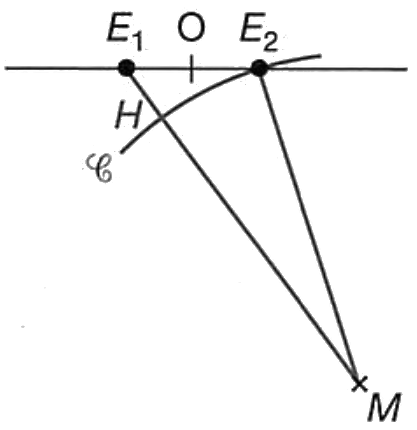
\includegraphics[width=0.2\linewidth]{cercle_corr-white}
            \end{center}
        \item E$_1$H est la différence ${\rm E_1M - E_2M} = r_1-r_2 = \D
            L_{1/2}(\Mr)$ avec les notations du cours~; autrement dit, c'est
            \fbox{la différence de marche} entre les deux ondes.
        \item En raisonnant dans le triangle $\rm E_1E_2H$, considéré rectangle, on
            a ${\rm E_1H} = a \sin\theta$. D'où le déphasage~:
            \[\boxed{\D\f_{2/1}(\Mr) = \frac{2\pi a\sin\theta}{\lambda}}\]
        \item L'amplitude est maximale pour des interférences constructives, soit
            pour $\D\f_{2/1}(\Mr) = 2p\pi$ avec $p\in\Zb$~; sur $\theta$ ça donne
            donc
            \[
                \boxed{\sin\theta = p \frac{\lambda}{a}}
                \Leftrightarrow
                \theta = \asin(p \frac{\lambda}{a})
            \]
            On regarde donc quels sont les ordres d'interférences $p$ tels que
            $\theta \in \SIrange{-30}{30}{\degree}$~:
            \begin{itemize}
                \item $p=0 \Rightarrow \theta = \ang{0;;}$, soit un maximum
                    pour tout l'axe $x$~: c'était attendu étant donné les symétries
                    du problème~;
                \item $p = \pm 1 \Rightarrow \theta = \pm\ang{12;;}$, donnant deux
                    points symétriques par rapport à (O$x$)~;
                \item $p = \pm 2 \Rightarrow \theta = \pm\ang{25;;}$, pratiquement
                    le double des valeurs précédentes.
            \end{itemize}
            $p > 2$ donne des valeurs en-dehors de l'intervalle.
    \end{enumerate}
    \item
        \begin{enumerate}
            \item On a interférences destructives si $\D\f_{2/1}(\Mr) =
                (2p+1)\pi$, soit
                \[
                    \boxed{\sin\theta = \left(p+\frac{1}{2}\right) \frac{\lambda}{a}}
                    \Leftrightarrow
                    \theta = \asin(\left(p+\frac{1}{2}\right) \frac{\lambda}{a})
                \]
                \begin{itemize}
                    \item $p=0 \Rightarrow \theta = \pm\ang{6;;}$~;
                    \item $p=1 \Rightarrow \theta = \pm\ang{19;;}$.
                \end{itemize}
            \item Pour des ondes reçues avec la même amplitude, l'opposition de
                phase conduit à une annulation totale de l'amplitude somme.
        \end{enumerate}
\end{enumerate}

\end{document}
